%%\documentclass[12pt,a4paper]{article}
%\usepackage[utf8]{inputenc}
%\usepackage[siunitx,american]{circuitikz}
%\usepackage{pgfplots}
%\usepackage[margin=0.5in]{geometry}
%\usepackage{textcomp}
%\usepackage[spanish, es-tabla]{babel}
%\usepackage{amsmath}
%\usepackage{graphicx}
%\usepackage[colorinlistoftodos]{todonotes}
%\usepackage{amsmath}
%\usepackage{float}
%\usepackage{makebox}
%\usepackage{tikz}
%\usetikzlibrary{arrows}
%\usetikzlibrary{shapes.misc}

%\usepackage{parskip}
%\usepackage{fancyhdr}
%\usepackage{vmargin}
%\setmarginsrb{3 cm}{2.5 cm}{3 cm}{2.5 cm}{1 cm}{1.5 cm}{1 cm}{1.5 cm}


%\pgfplotsset{compat=1.15}
%\setlength{\parindent}{12pt}

%\begin{document}
\section{Filtro Notch}
\subsection{Análisis del circuito}
En este ejercicio se busca crear un filtro notch a partir del circuito \ref{fig:circuito_1}. 

\begin{figure}[H]                                                       
    \centering
    	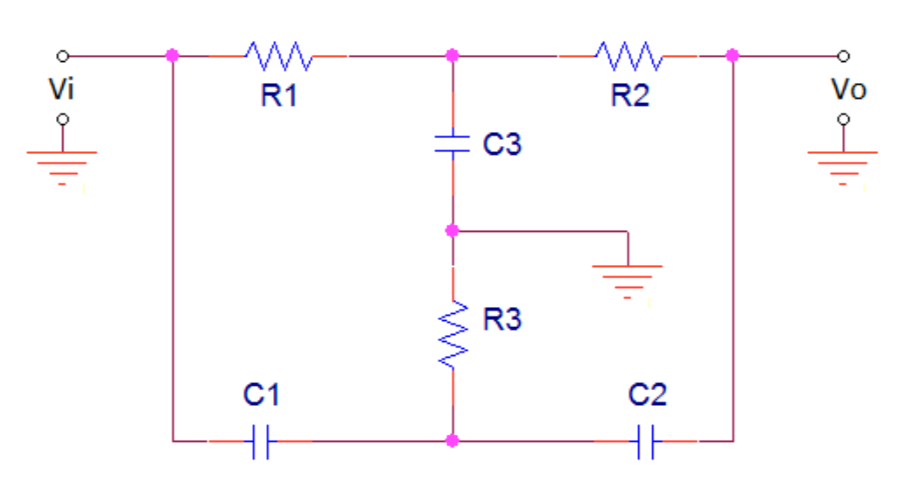
\includegraphics[width=0.5\textwidth]{resources/circuito_1.png}
    	\caption{Filtro Notch Pasivo}
    	\label{fig:circuito_1}
\end{figure}

En una primera instancia a través del uso de la herramienta matlab se logró conseguir la función transferencia a través de la resolución de un sistema de ecuaciones, en una segunda instancia se transformaron ambos circuitos tipo T en circuitos tipo PI mediante el teorema de Kennely y se consiguió el circuito de la figura \ref{circuitoconkenelly}.

\begin{figure}[H]                                                       
    \centering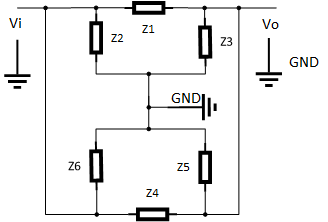
\includegraphics[width=0.4\textwidth]{resources/circuitoconkenelly.png}
    \caption{Mismo circuito con el teorema de Kenelly aplicado}
    \label{circuitoconkenelly}
\end{figure}
Se notó que $Z2$ y $Z6$ se encontraban en paralelo, de la misma manera lo estaban $Z3$ con $Z5$ y $Z1$ con $Z4$, por lo que se prosiguió a calcular el equivalente y se obtuvo el circuito de la figura \ref{circuitoconkenellysimplificado}.

\begin{figure}[H]                                                       
    \centering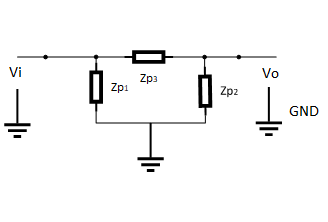
\includegraphics[width=0.5\textwidth]{resources/circuitoconkenellysimplificado.png}
    \caption{Circuito con el teorema de Kenelly aplicado simplificado}
    \label{circuitoconkenellysimplificado}
\end{figure}

Con los valores:
\begin{equation}
Z_{p1}=Z_{p2}=\dfrac{C_3 \ R_3 \ s + \ 1}{C_3 \ s} \ \ ; \ Z_{p3}=\dfrac{4 \ R_3 \ (C_3 \ R_3 \ s \ + \ 1)}{C_3^2 \ R_3^2 \ s^2 \ + \ 1}
\end{equation}
Una vez se llegó a este punto fue más fácil encontrar la función transferencia y se obtuvo lo detallado en la ecuación \ref{transferencia_1}.
%En primer lugar, se calculó analíticamente al circuito mediante un método alternativo como es el de cuadripolos para obtener la función transferencia $H(s)$ que se puede ver en la ecuación \ref{transferencia_1}.
Vale aclarar que se utilizó la ayuda propuesta por la cátedra y se consideró que $R_{1} = R_{2}
= 2 \ R_{3}$ y $2 \ C_{1} = 2 \ C_{2} = C_{3}$.

\begin{equation} H(s) = \frac{(\frac{S}{1/C_{3} R_{3}})^2 + 1} {(\frac{S}{1/C_{3}R_{3}})^2 + 4\frac{S}{C_{3}R_{3}} + 1}  \label{transferencia_1}\end{equation}.

Como se puede observar, la función transferencia describe un filtro Notch. Su frecuencia de corte es
$W_0$ y su expresión se muestra en la ecuación \ref{frecuencia_corte}.

\begin{equation} W_{0} =  \frac{1}{C_{3} R_{3}}  \label{frecuencia_corte}\end{equation}

La frecuencia de corte pedida es $10.8k Hz$, obtenemos así la relación que se puede ver en la ecuación \ref{relacion_RC}.

\begin{equation} R_{3} = \frac{1}{C_{3} \  2 \ \pi \ 10.8k} \label{relacion_RC}\end{equation}

Es posible dar valores al capacitor y así obtener un valor para las resistencias. Teniendo en cuenta los valores comerciales disponibles en el pañol, se tomo $C_{3} = 10nF$ y se obtuvo $R_{3}=1.47k\Omega$. Al no haber disponibilidad de una resistencia fija de ese valor, se utilizo una $R_{3}=1.5k\Omega$. Tampoco se encontraron capacitores de $C = 5nF$ por lo que se utilizaron tanto $C_{1} = 4.7nF$ como  $C_{2} = 4.7nF$. Estos valores se cargaron en LTspice y se obtuvo el bode de la figura \ref{fig:bode_ltspice_teorico}.

%\begin{figure}[H]                                                       
%    \centering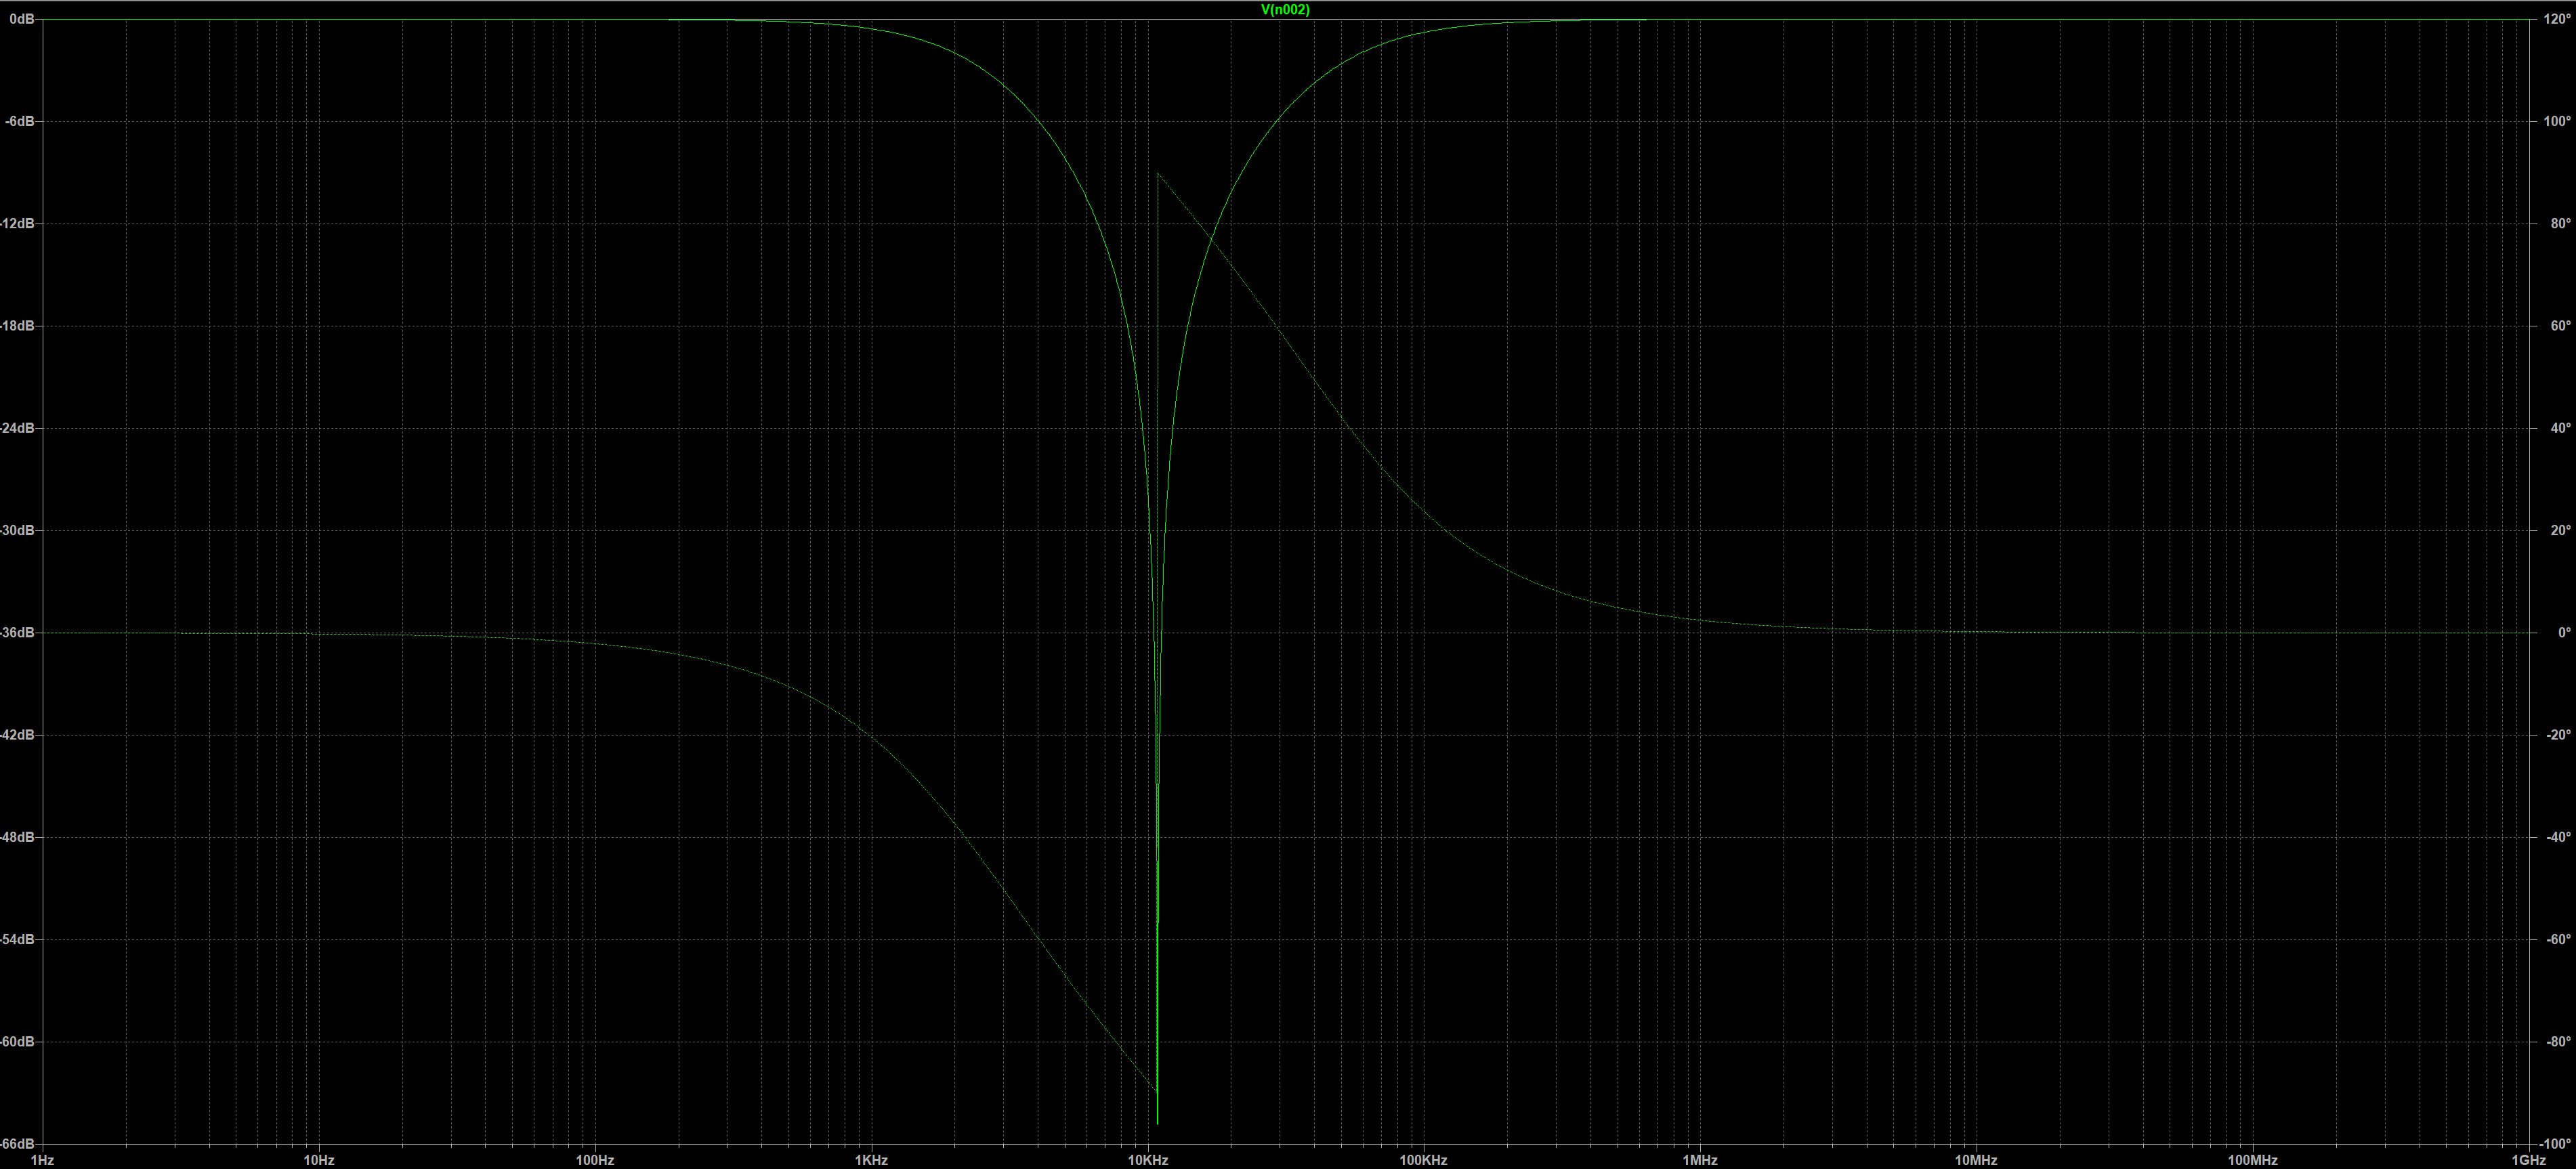
\includegraphics[width=\paperwidth, height=\textheight,keepaspectratio]{bode_ltspice_teorico.png}
%    \caption{Circuito con los componentes definidos}
%    \label{fig:bode_ltspice_teorico}
%\end{figure}

\begin{figure}[H] 
\begin{center}
\makebox[\textwidth]{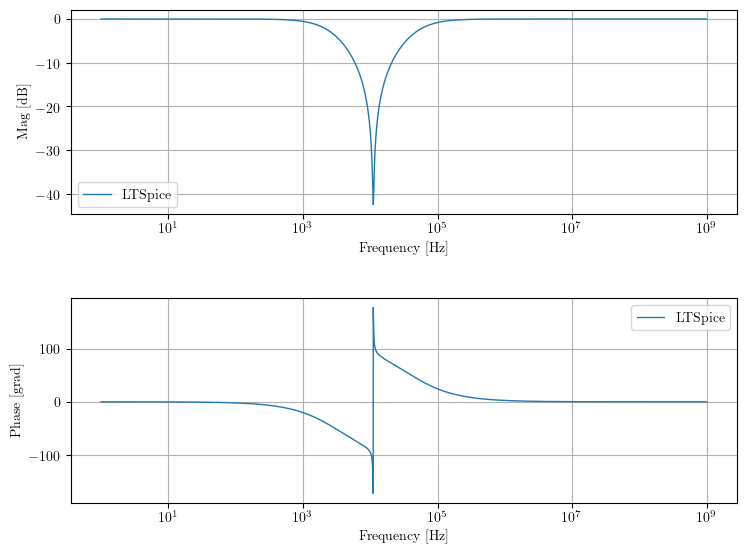
\includegraphics[width=\paperwidth, height=\textheight,keepaspectratio]{resources/bode_ltspice_teorico2.png}}
\caption{Circuito con los componentes definidos}
\label{fig:bode_ltspice_teorico}
\end{center}
\end{figure}

Se puede observar que el comportamiento del bode describe un filtro notch y que la frecuencia de corte se ubica en $11.1kHz$. Si
bien la frecuencia de corte pedida es $10.8kHz$ nos vemos obligados a tomar $11.1kHz$ por motivos de disponibilidad de componentes
en el pañol. Luego las futuras mediciones se comparan respecto al bode obtenido en la figura \ref{fig:bode_ltspice_teorico}. \\

Para obtener la respuesta impulsiva $h(t)$, se utilizó la antitrasformada de Laplace conseguida mediante el uso de matlab. Esta resulto ser la que se muestra en la ecuación \ref{ecuacionrtaimpulsiva} y se puede ver graficada en la figura \ref{respuestaimpulsiva} .

\begin{equation}
y \! \left(t\right) = \delta \! \left(t\right) - \dfrac{4\, \mathrm{e}^{-\frac{2\, t}{\mathrm{C3}\, \mathrm{R3}}}} {\mathrm{C3}\, \mathrm{R3}} \left(\cosh\!\left(\dfrac{\sqrt{3}\, t}{\mathrm{C3}\, \mathrm{R3}}\right) - \dfrac{2\, \sqrt{3}\, \sinh\!\left(\dfrac{\sqrt{3}\, t}{\mathrm{C3}\, \mathrm{R3}}\right)}{3}\right)
\label{ecuacionrtaimpulsiva}
\end{equation}

\begin{figure}[H] 
\begin{center}
\makebox[\textwidth]{\includegraphics[width=\paperwidth, height=\textheight,keepaspectratio]{resources/respuestaimpulsiva.png}}
\caption{Respuesta impulsiva}
\label{respuestaimpulsiva}
\end{center}
\end{figure}

%\begin{equation} 
%h_{t} = \delta \! \left( t \right) - 4\, w\, \mathrm{e}^{-2\, t\, w} \left(\cosh\!\left(\sqrt{3}\, t\, w\right) - \dfrac{2\, \sqrt{3}\, \sinh\!\left(\sqrt{3}\, t\, w\right)}{3}\right)
%\end{equation}

    %dirac(t) - 4*w*exp(-2*t*w)*(cosh(3^(1/2)*t*w) - (2*3^(1/2)*sinh(3^(1/2)*t*w))/3)

%\begin{figure}[H]                                                       
%    \centering\includegraphics[width=0.8\textwidth]{respuestaimpulsiva.png}
%    \caption{Respuesta impulsiva}
%    \label{circuitoconkenellysimplificado}
%\end{figure}


Por último para poder terminar de caracterizar el sistema hace falta el diagrama de polos y ceros. Los polos y ceros se obtienen fácilmente si reordenamos la función transferencia como se ve continuación:

\begin{center}
    $H(S) = \dfrac{(S-S_{1})(S-S_{2})}{(S-P_{1})(S-P_{2})S}$  \\
\end{center}

Hay dos ceros:
\begin{center}
    $S_{1}=69743.35691j $
    $S_{2}=-69743.35691j $
    \end{center}

Hay dos polos:

\begin{center}
    $P_{1}=-18687.67616$
    $P_{2}=-260285.7515$
\end{center}

Como se puede ver los dos ceros se encuentran sobre el eje imaginario y los dos polos en el eje real del semilado negativo


\begin{center}\begin{tikzpicture}
    %\draw   (5,0) -- (-5, 0)
    %        (0,5) -- (0,-5);
	\draw [-latex] (-5,0) -- (5,0) node [above left]  {$\Re$};  %Eje X
	\draw [-latex] (0,-5) -- (0,5) node [below right] {$\Im$};  %Eje Y
	\node[cross out,draw=red] at (0,4.5)[label={[label distance=1pt,red]0:S1}] {};
    %\draw   [red, thick](0,0) -> (0,4.5) node[anchor=north east] {S1};
   	\node[cross out,draw=red] at (0,-4.5)[label={[label distance=1pt,red]0:S2}] {};
    %\draw   [red, thick](0,0) -> (0,-4.5) node[anchor=north east] {S2};
	\node[circle,draw=blue] at (-1,0)[label={[label distance=1pt,blue]270:P1}] {};
    %\draw   [blue, thick](0,0) -> (-1,0) node[anchor=north east] {P1};
   	\node[circle,draw=blue] at (-2,0)[label={[label distance=1pt,blue]270:P2}] {};
    %\draw   [blue, thick](0,0) -> (-2,0) node[anchor=north east] {P2};
    \end{tikzpicture}
    \end{center}

\subsection{Respuesta en frecuencia}
Con los valores de los componentes calculados anteriormente, se diseño una placa en Altium. Su diseño se 
puede ver en la figura \ref{fig:placa_altium}.

\begin{figure}[H]                                                       
    \centering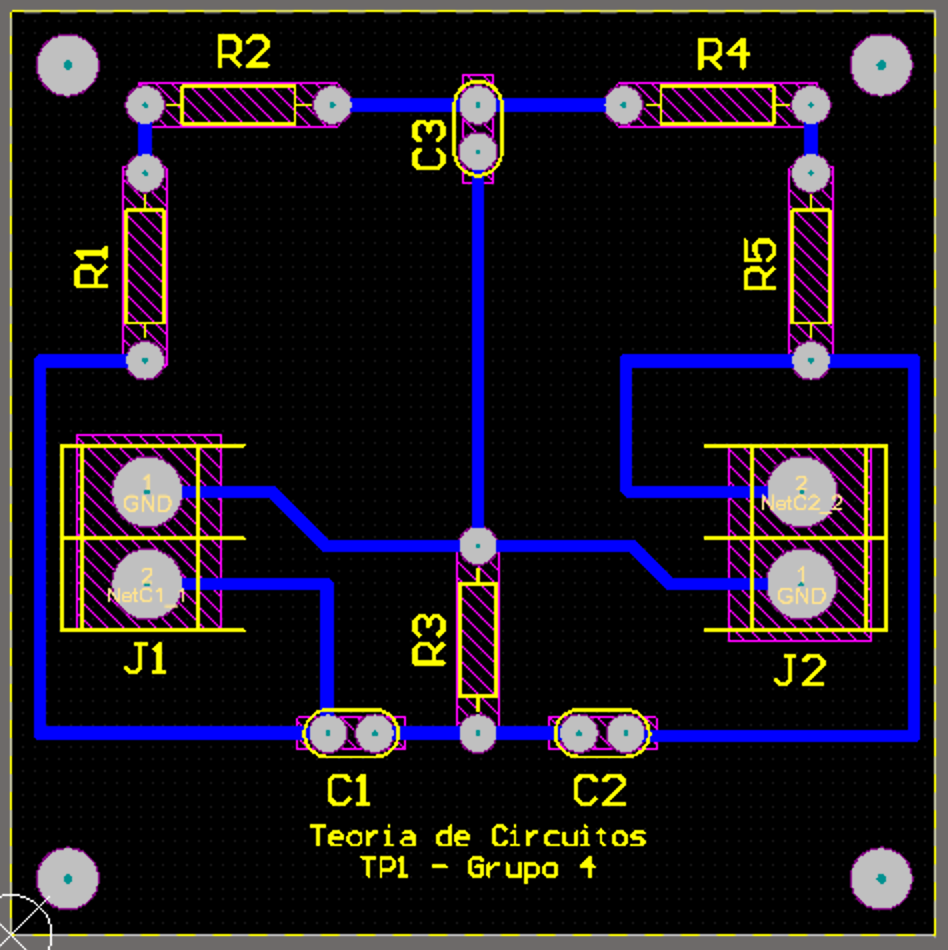
\includegraphics[width=0.3\textwidth]{resources/placa_altium.png}
    \caption{Placa diseñada en Altium}
    \label{fig:placa_altium}
    \end{figure}

Notar que se utilizaron que utilizar dos resistencias en serie de $1.5k\Omega$ para obtener una
resistencia de $3k\Omega$. 

Para medir la respuesta en frecuencia se utilizo un generador de señales y se alimento al circuito con un senoide en $V_{in}$ y se midió $V_{out}$ con la ayuda de un osciloscopio.

En primer lugar se excito el circuito con una señal senoidal de $10 \ V_{pp}$ a una frecuencia de $11.1kHz$, que es la frecuencia de corte buscada con nuestros componentes. Se esperaría ver una señal totalmente atenuada ya que la señal de entrada esta en la frecuencia de corte. Se realizó un barrido rápido en las frecuencias cercanas a $11.1kHz$ y notamos que nuestro filtro tenía la mayor atenuación en $11.3kHz$. Los resultados fueron los siguientes: $V_{in}=9,73V$ y $V_{out}= 0,038V$ lo que da una atenuación de $20\log(\dfrac{V_{out}}{V_{in}}) = -48,16db$ , representando la salida tan sólo el $0.39 \%$ de la entrada. 

Podemos decir que se puede considerar que la señal de entrada fue totalmente atenuada a esta frecuencia y que
%Si hacemos el calculo de atenuación esta da $20\log(\dfrac{V_{out}}{V_{in}}) = -48,16db$. Esta atenuación debería serla mas chica cuando se realice el bode completo. 
hay que tener en cuenta el ruido, el 
osciloscopio es susceptible al ruido. Esto explica porque $V_{out}$ no es cero en la frecuencia de corte del Notch. Lo que se esta midiendo en esta situación es prácticamente ruido ya que este tiende a aumentar al ser tan pequeña la amplitud de la señal. \\

Si tenemos en cuenta que la frecuencia de corte que se planeaba obtener con los componentes elegidos y la que obtuvimos, el filtro fabricado tiene un error un $1.82 \ \%$. Y si se compara con los $10.8 \ kHz$ que se buscaban en un comienzo, este error es de un $4.63 \ \%$.

Se prosiguió a realizar el bode completo. Para esto se mantuvo una senoide de $10 \ V_{pp}$ pico a pico
y se fue modificando la frecuencia de esta. Sabiendo de antemano como es la curva que 
describe el bode, se tomaron mas puntos en las áreas mas características del bode. Como lo es el área cercana a la frecuencia de corte. Los resultados del bode completo se pueden ver en la figura \ref{fig:superpuesto}.

\begin{figure}[H] 
\begin{center}
\makebox[\textwidth]{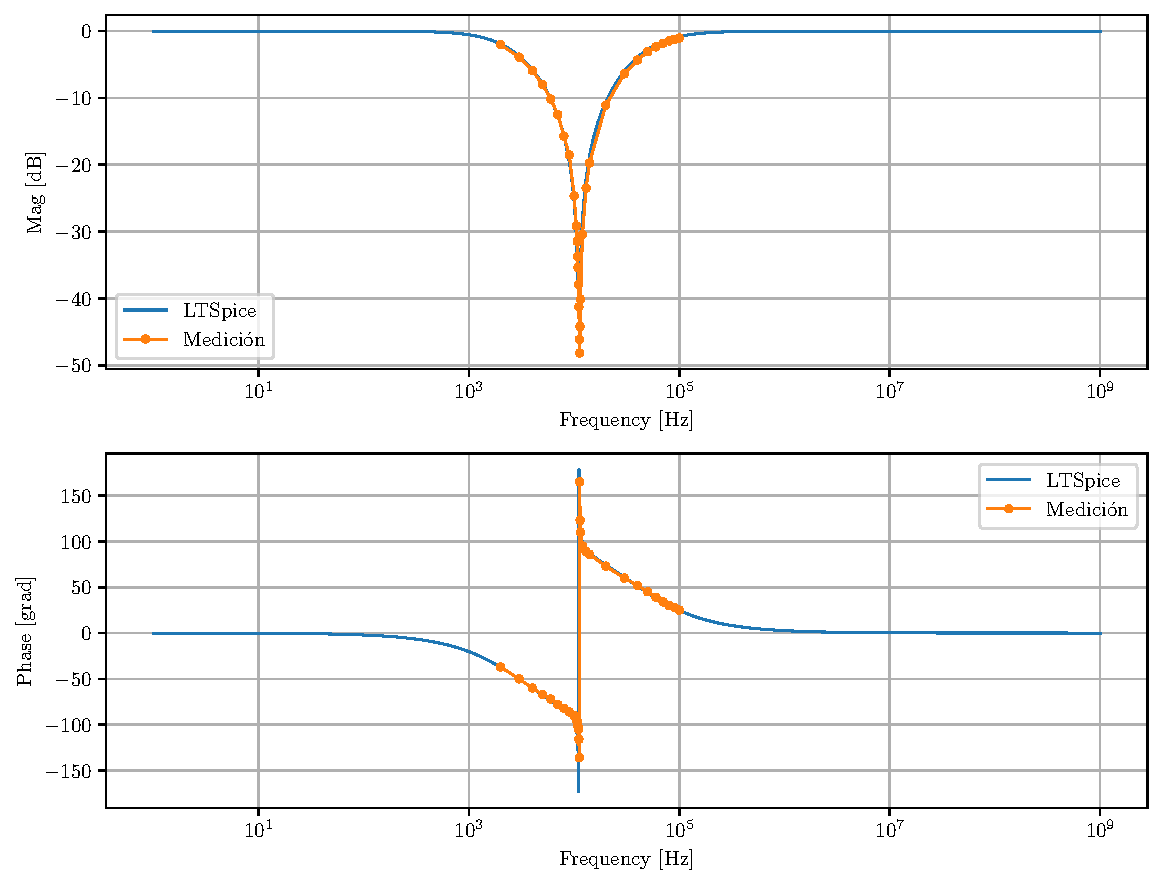
\includegraphics[width=\paperwidth, height=\textheight,keepaspectratio]{resources/Superpuesto.pdf}}
\caption{Filtro Notch Pasivo}
\label{fig:superpuesto}
\end{center}
\end{figure}

%\begin{figure}[H]                                                       
%    \centering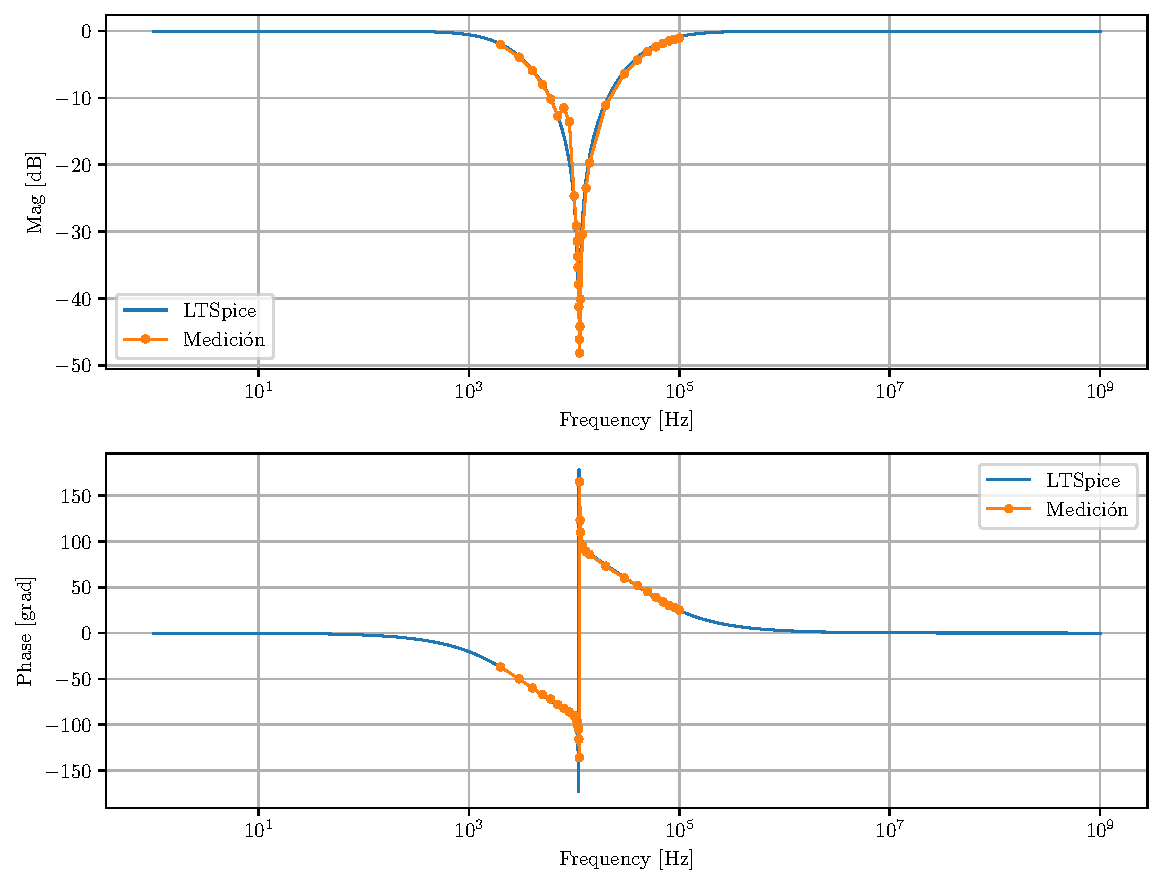
\includegraphics[width=0.8\textwidth]{Superpuesto.pdf}
%    \caption{Filtro Notch Pasivo}
%    \label{fig:superpuesto}
%\end{figure}

Como se puede observar, la figura \ref{fig:superpuesto} tiene superpuesto el bode
de LTspice (curva azul) que se mostró en la figura \ref{fig:bode_ltspice_teorico} y el bode que se obtuvo de forma experimental (curva naranja). Los resultados son sumamente satisfactorios. En el bode de la medición se puede apreciar la frecuencia de corte y como el resto de los puntos se asemejan a la curva teórica calculada en LTspice. 


\subsection{Respuesta al escalón}
%En esta parte se analizó la respuesta al escalón. En primer lugar se calculo la expresión analítica. Teniendo en cuenta que la entrada $X(t)$ es el escalón $U(t)$, que su transformada de Laplace es $\frac{1}{S}$ y que la función transferencia es la que vimos en la ecuacion \ref{transferencia_1}. La transformada de Laplace de la salida nos queda \ref{transferencia_2}


%\begin{equation} Y(S) = \dfrac{S^2+W_{0}^2}{S^2+4W_{0}S+W_{0}^2} * \dfrac{1}{S}  \label{transferencia_2}\end{equation}

%Si acomodamos un poco esta expresion podemos llegar a: \\

%\begin{center}
%\begin{equation}
%    Y(S) = \dfrac{(S-S_{0})(S+S_{0})}{(S-P_{1})(S-P_{2})S}
%\end{equation}

%    $S_{0}=69743.35691j
%    P_{1}=-18687.67616
%    P_{2}=-260285.7515$
%    \end{center}

%Si antitrasformamos nos queda:\\

%\begin{center}
%    $y(t) = (A\exp{P_{1}t}+B\exp{P_{2}t}+C) * u(t)$

%    $A = \dfrac{P_{1}^2 + W_{0}^2}{(P_{1}-P_{2})*P_{1}} = -1.1547$
%    $B = \dfrac{P_{2}^2 + W_{0}^2}{(P_{2}-P_{1})*P_{2}} =  1.1547$
%    $C = \dfrac{W_{0}^2}{(P_{2}P_{1}} = 1$

%    \end{center}

Para la obtención de la respuesta teórica al escalón se realizó lo mismo que se mencionó anteriormente para la respuesta al impulso y se muestra a continuación en la ecuación \ref{ecuacionrtaalescalon} su resultado y en la figura \ref{respuestaalescalon} su gráfico.

\begin{equation}
y \! \left(t\right) = 1 - \dfrac{4}{3}\, \sqrt{3}\, \mathrm{e}^{-\frac{2\, t}{\mathrm{C3}\, \mathrm{R3}}}\, \sinh\!\left(\dfrac{\sqrt{3}\, t}{\mathrm{C3}\, \mathrm{R3}}\right)
\label{ecuacionrtaalescalon}
\end{equation}

\begin{figure}[H] 
\begin{center}
\makebox[\textwidth]{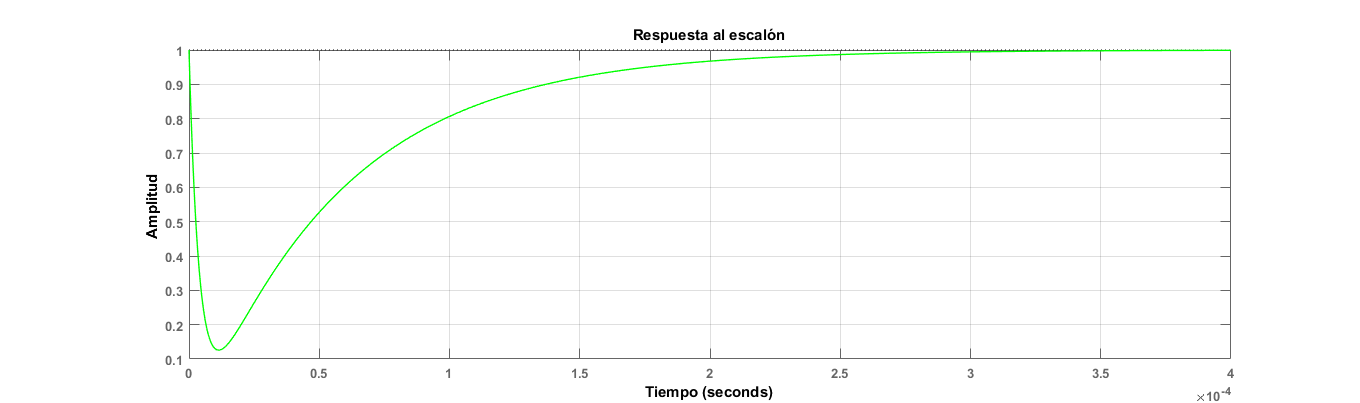
\includegraphics[width=\paperwidth, height=\textheight,keepaspectratio]{resources/respuestaalescalon.png}}
\caption{Respuesta al escalón}
\label{respuestaalescalon}
\end{center}
\end{figure}

%Si simulamos en LTspice la respuesta al ecalon tomando $C_{3} = 10nF$ y $R_{3}=1.47k\Omega$, nos queda los que observamos en 
%la figura \ref:fig{rta_escalon_teorica}

%\begin{figure}[ht]                                                       
%    \centering\includegraphics[width=0.8\textwidth]{rta_escalon_teorica.png}
%    \caption{Respuesta al Escalón}
%    \label{fig:rta_escalon_teorica}
%    \end{figure}

A continuación en la figura \ref{rtaalescalonosciloscopio} se muestra la imagen tomada del osciloscopio al momento de excitar el circuito con el escalón:

\begin{figure}[H]                                                       
    \centering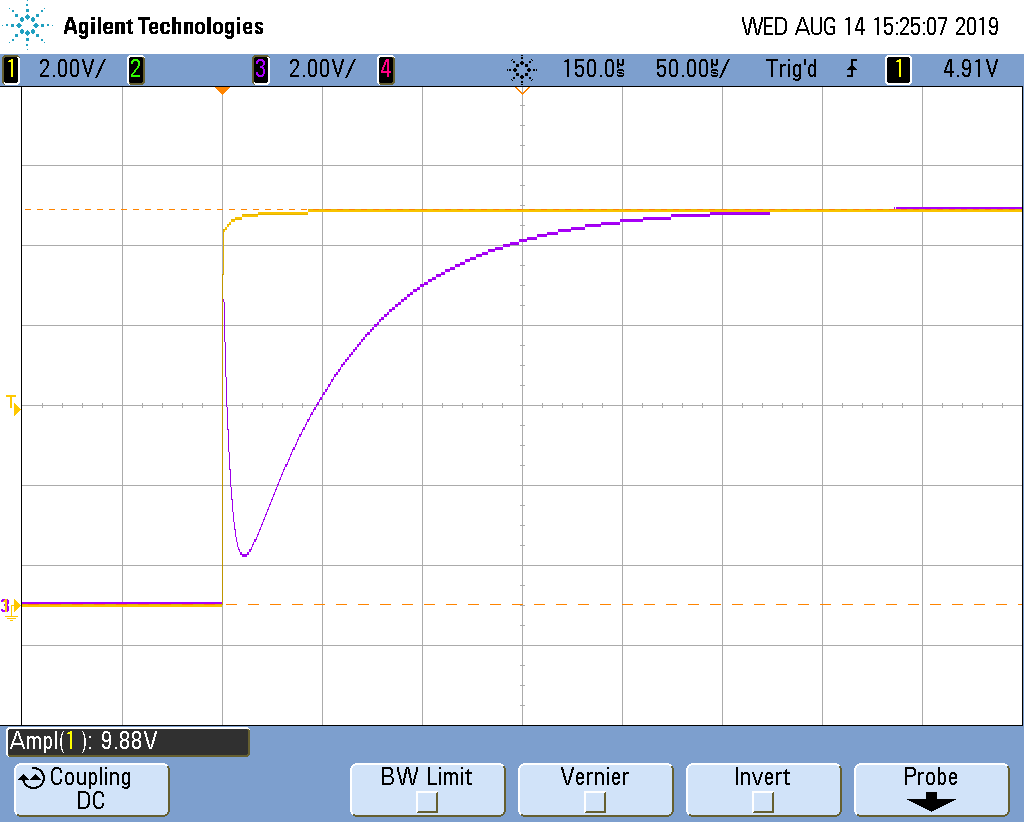
\includegraphics[width=\textwidth]{resources/rtaalescalon.png}
    \caption{Respuesta al escalón medida}
\label{rtaalescalonosciloscopio}
\end{figure}

La línea violeta es la repuesta al escalón  medida y la amarilla es el escalón. Podemos decir entonces  que se corresponde de manera adecuada la respuesta medida con la teórica y que el circuito se comportó como se esperaba.
 
%\end{document}